\documentclass[10pt,a4paper, margin=1in]{article}
\usepackage{fullpage}
\usepackage{amsfonts, amsmath, pifont}
\usepackage{amsthm}
\usepackage{graphicx}
\usepackage{float}

\usepackage{tkz-euclide}
\usepackage{tikz}
\usepackage{pgfplots}
\pgfplotsset{compat=1.13}

\usepackage{geometry}
 \geometry{
 a4paper,
 total={210mm,297mm},
 left=10mm,
 right=10mm,
 top=10mm,
 bottom=10mm,
 }
 % Write both of your names here. Fill exxxxxxx with your ceng mail address.
 \author{
  YILMAZ, Mert Kaan\\
  \texttt{e2381093@ceng.metu.edu.tr}
}

\title{CENG 384 - Signals and Systems for Computer Engineers \\
Spring 2022 \\
Homework 1}
\begin{document}
\maketitle



\noindent\rule{19cm}{1.2pt}

\begin{enumerate}

\item %write the solution of q1
    \begin{enumerate}
    % Write your solutions in the following items.
    \item To use $\Bar{z}$ in equation, first we need to find it by taking the conjugate of z.\\
    $\Bar{z} = x - yj$\\
    Now we can put corresponding values into given equation.\\
    $2(x + yj) - 9 = 4j - (x - yj)$\\
    $3x + yj = 9 + 4j$\\
    Therefore $x = 3$ and $y = 4$\\
    Put x and y values in z, we get: $z = 3 + 4j$\\
    $|z| = \sqrt{(3)^2 + (4)^2} = 5$ \\
    $|z|^2 = 25$ \\
    z on the complex plane:
    \begin{figure}[h!]
    \centering
        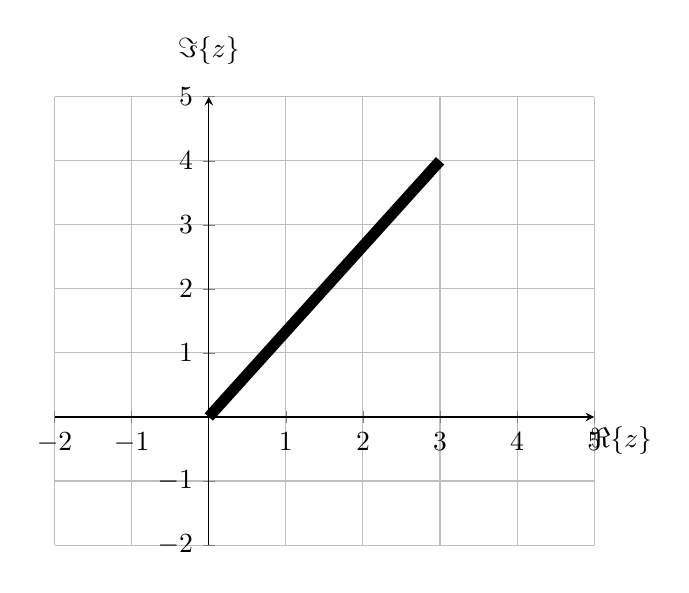
\begin{tikzpicture}[scale=1.0]
          \begin{axis}[
          axis lines=middle,
          xlabel={$\Re\{z\}$},
          ylabel={$\Im\{z\}$},
          xtick={-2, -1, ..., 5},
          ytick={-2, -1, ..., 5},
          ymin=-2, ymax=5,
          xmin=-2, xmax=5,
          every axis x label/.style={at={(ticklabel* cs:1.05)}, anchor=north,},
          every axis y label/.style={at={(ticklabel* cs:1.05)}, anchor=south,},
          grid,
        ]
          \path[draw,line width=4pt] (0,0) -- (3,4);
          \end{axis}
        \end{tikzpicture}
        \caption{$z = 3 + 4j$}
        \label{fig:fig1}
    \end{figure}
    
    \item
    We know $z = re^{j \theta }$\\
    and $z^3 = -27j$ is given.\\
    Therefore, $r^3e^{3j \theta} = -27j$\\
    From this equation, we can find that\\
    $r = -3$, \\
    $e^{3j \theta } = j$ \\
    From Euler's Formula:\\
    $e^{j(3 \theta) } = \cos{( \frac{ \pi }{2})} + j \sin{(\frac{ \pi }{2})} = j$ \\
    So,\\
    $3 \theta = \frac{ \pi }{2}$ then $ \theta = \frac{ \pi }{6}$ \\
    Now let's write z in polar form\\
    $z = -3\cdot( \cos{( \frac{ \pi }{6}}) + j \sin{( \frac{ \pi }{6})})$ \\
    $z = -3e^{(j\frac{ \pi }{6} + \frac{2 \pi }{3} m)}$ for m=1,2,3,... \\
    \newpage
    \item Multiply both denominator and numerator with conjugate of $\sqrt{3}+j$\\
    $z = \frac{(1 + j)(\sqrt{3} - j)^2}{(\sqrt{3} + j)(\sqrt{3} - j)} = \frac{(1 + j)(\sqrt{3} - j)^2}{2} = 2 + \sqrt{3} - j\sqrt{3} + 2j $ \\
    Magnitude of z:\\
    $\sqrt{(2+\sqrt{3})^2+(2-\sqrt{3})^2} = \sqrt{14}$\\
    Angle of z:\\
    $ \theta = \arctan{( \frac{2-\sqrt{3}}{2+\sqrt{3}} )} = 4.1074 degrees$ \\
    \item $z = -(1+j)^8e^{j\frac{\pi}{2}}$ is given.\\
    $z = -(1+j)^8e^{j\frac{\pi}{2}}$ = $z = -(2j)^4e^{j\frac{\pi}{2}}$ = $z = -16e^{j\frac{\pi}{2}}$\\
    \end{enumerate}

\item %write the solution of q2
    \begin{enumerate}
    % Write your solutions in the following items.
    \item Energy: E = $\sum_{n=-\infty}^{\infty} \vert nu[n]\vert$ \\
    E = $\sum_{n=-\infty}^{-1}0$ + $\sum_{n=0}^{\infty}n$ = $0 + 1 + 2 + 3 + ...$ \\
    E = $\infty$ which does not hold $0 < E < \infty$. Therefore it's not an energy signal. \\
    Power: P = $\lim_{N\to\infty} \frac{1}{2N+1} [\sum_{n=-N}^{N} \vert nu[n]\vert]$ \\
    P = $\lim_{N\to\infty} \frac{1}{2N+1} [\sum_{n=0}^{N} \vert n\vert]$ \\
    P = $\infty$ = $\lim_{N\to\infty} \frac{N(N+1)}{2(2N+1)} $ \\
    Therefore P is not a power signal. \\
    To conclude, we can say that the signal x[n] is neither energy nor power signal.
    \item Energy: E = $\lim_{T\to\infty}\int_{-T}^{T} (e^{-2t})^2u(t)dt$ = $\lim_{T\to\infty}\int_{0}^{T} (e^{-4t})dt$ \\
    E = $\lim_{T\to\infty}\frac{e^{-4t}}{-4}\rvert_{0}^{T}$ = $\lim_{T\to\infty}(\frac{e^{-4T}}{-4} + \frac{1}{4})$ \\
    E = $\frac{1}{4}$. Since equation $0 < E < \infty$ holds, we can say that it's an energy signal. \\
    Power: P = $\lim_{T\to\infty}\frac{(\frac{e^{-4t}}{-4} + \frac{1}{4})}{2T}$ = $0$ and since P=0, it's not a power signal. \\
    Conclusion: signal x(t) is an energy signal but not a power signal.
    \end{enumerate}

\item The signal of $y(t) = \frac{1}{2}x(-\frac{1}{3}t+2)$ \\
    \begin{figure}[h!]
    \centering
        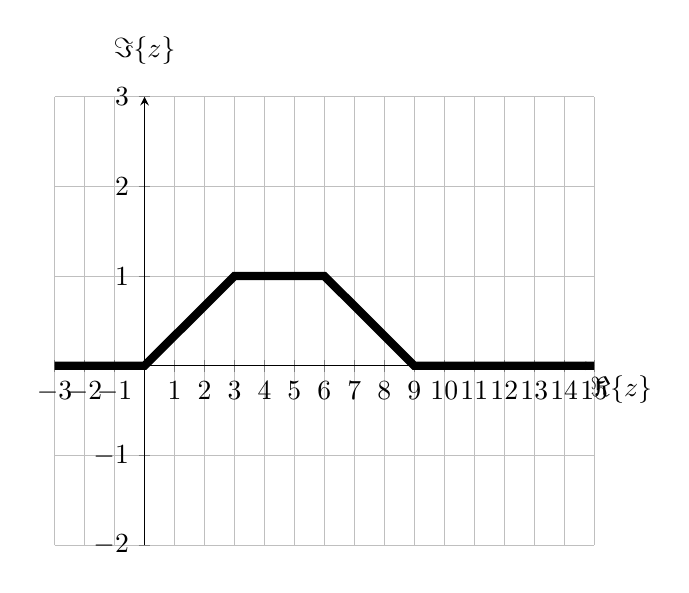
\begin{tikzpicture}[scale=1.0]
          \begin{axis}[
          axis lines=middle,
          xlabel={$\Re\{z\}$},
          ylabel={$\Im\{z\}$},
          xtick={-3, -2, ..., 15},
          ytick={-2, -1, ..., 3},
          ymin=-2, ymax=3,
          xmin=-3, xmax=15,
          every axis x label/.style={at={(ticklabel* cs:1.05)}, anchor=north,},
          every axis y label/.style={at={(ticklabel* cs:1.05)}, anchor=south,},
          grid,
        ]
          \path[draw,line width=3pt] (-3,0) -- (0,0) -- (3,1) -- (6,1) -- (9,0) -- (15,0);
          \end{axis}
        \end{tikzpicture}
        \caption{$y(t) = \frac{1}{2}x(-\frac{1}{3}t+2)$}
        \label{fig:fig1}
    \end{figure}

\begin{filecontents}{fig3.dat}
 n   xn
 -4  0
 -3  2
 -2  0  
 -1  2
  0  -1
 1   -3 
 2   0
 3   0
 4   1
\end{filecontents}

\newpage
\item %write the solution of q4
    \begin{enumerate}
    % Write your solutions in the following items.
    \item To get $x[-2n]$, we simply take symmetry wrt. y axis and shrink it by 2.\\
    For $x[n-2]$, we move the graph by 2 to right.\\
    After those steps, we sum them up and draw $x[-2n] + x[n-2]$\\
        \begin{figure}[h!]
            \centering
            \begin{tikzpicture}[scale=1.0] 
              \begin{axis}[
                  axis lines=middle,
                  xlabel={$n$},
                  ylabel={$x[-2n] + x[n-2]$},
                  xtick={ -4, -3,  ..., 5},
                  ytick={-3, -2, -1, ..., 3},
                  ymin=-3, ymax=3,
                  xmin=-5, xmax=5,
                  every axis x label/.style={at={(ticklabel* cs:1.05)}, anchor=west,},
                  every axis y label/.style={at={(ticklabel* cs:1.05)}, anchor=south,},
                  grid,
                ]
                \addplot [ycomb, black, thick, mark=*] table [x={n}, y={xn}] {fig3.dat};
              \end{axis}
            \end{tikzpicture}
            \caption{$n$ vs. $x[-2n] + x[n-2]$.}
            \label{fig:fig2}
        \end{figure}
    \item $x[-2n] + x[n-2]$ = $2\delta(n+3) + 2\delta(n+1) - \delta(n) -3\delta(n-1) + \delta(n-4)$
    \end{enumerate}

\item %write the solution of q5
    \begin{enumerate}   
    % Write your solutions in the following items.
    \item It's periodic.\\
    $\frac{e^{j3t}}{-j} = \frac{e^{j3(t+T)}}{-j}$ \\
    $\frac{e^{j3t}}{-j} = \frac{e^{j3(t)}}{-j}\cdot e^{j3(T)}$ \\
    $e^{j3(T)}=1$ \\
    Since $e^{2\pi k} = 1$ and $e^{j3(T)} = e^{2\pi k}$ we can say that $2\pi k = 3T$ \\
    Therefore $T = \frac{2\pi k}{3}$ for all k. \\
    The fundamental period is the smallest positive value for k, so we can put 1 at k to get the fundamental period as $T_0 = \frac{2\pi}{3}$.
    \item It's periodic.\\
    Let's say $\frac{1}{2}sin[\frac{7\pi}{8}n] + 4cos[\frac{3\pi}{4}n - \frac{\pi}{2}] = x_1[n] + x_2[n]$,\\
    $x_1[n] = \frac{1}{2}sin[\frac{7\pi}{8}n]$ and $x_2[n] = 4cos[\frac{3\pi}{4}n - \frac{\pi}{2}]$\\
    So,\\
    For $x_1$: \\
    $\frac{1}{2}sin[\frac{7\pi}{8}n] = \frac{1}{2}sin[\frac{7\pi}{8}(n+N)]$ \\
    $\frac{7\pi}{8}n + 2\pi k = \frac{7\pi}{8}n + \frac{7\pi}{8}N$ \\
    $N = \frac{16k}{7}$ for k=7,14,21... \\
    Then $N_1$ = 16. \\
    For $x_2$: \\
    $4cos[\frac{3\pi}{4}n - \frac{\pi}{2}] = 4cos[\frac{3\pi}{4}(n+N) - \frac{\pi}{2}]$ \\
    $\frac{3\pi}{4}n - \frac{\pi}{2} + 2\pi k = \frac{3\pi}{4}n + \frac{3\pi}{4}N - \frac{\pi}{2}$ \\
    $N = \frac{8k}{3}$ for k=3,6,9... \\
    Then $N_2$ = 8. \\
    Fundamental period = $N_0$ = LCM(16, 8)= 16
    \end{enumerate}

\newpage
\item %write the solution of q6
    \begin{enumerate}
    % Write your solutions in the following items.
    \item Because the signal is not symmetric about the origin, we can say that it's not odd. Additionally, since the signal is not symmetric about the y-axis, it's not an even signal either. Therefore, we can conclude that the signal is neither even nor odd.
    \item Even decomposition: $Even\{x(t)\} = \frac{(x(t)+x(-t))}{2}$\\
    Odd decomposition: $Odd\{x(t)\} = \frac{(x(t)-x(-t))}{2}$\\
    \begin{figure}[h!]
    \centering
        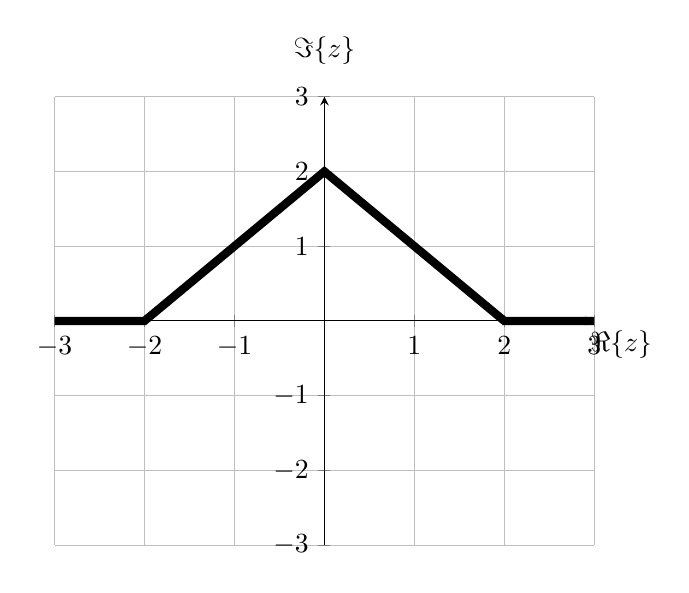
\begin{tikzpicture}[scale=1.0]
          \begin{axis}[
          axis lines=middle,
          xlabel={$\Re\{z\}$},
          ylabel={$\Im\{z\}$},
          xtick={-3, -2, ..., 3},
          ytick={-3, -2, ..., 3},
          ymin=-3, ymax=3,
          xmin=-3, xmax=3,
          every axis x label/.style={at={(ticklabel* cs:1.05)}, anchor=north,},
          every axis y label/.style={at={(ticklabel* cs:1.05)}, anchor=south,},
          grid,
        ]
          \path[draw,line width=3pt] (-3,0) -- (-2,0) -- (0,2) -- (2,0) -- (3,0);
          \end{axis}
        \end{tikzpicture}
        \caption{$Even\{x(t)\} = \frac{(x(t)+x(-t))}{2}$}
        \label{fig:fig1}
    \end{figure}
    
    \begin{figure}[h!]
    \centering
        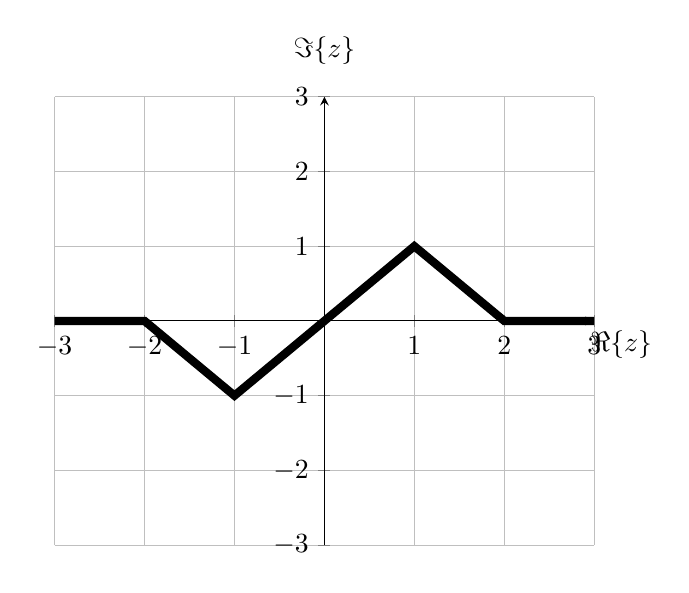
\begin{tikzpicture}[scale=1.0]
          \begin{axis}[
          axis lines=middle,
          xlabel={$\Re\{z\}$},
          ylabel={$\Im\{z\}$},
          xtick={-3, -2, ..., 3},
          ytick={-3, -2, ..., 3},
          ymin=-3, ymax=3,
          xmin=-3, xmax=3,
          every axis x label/.style={at={(ticklabel* cs:1.05)}, anchor=north,},
          every axis y label/.style={at={(ticklabel* cs:1.05)}, anchor=south,},
          grid,
        ]
          \path[draw,line width=3pt] (-3,0) -- (-2,0) -- (-1,-1) -- (1,1) -- (2,0) -- (3,0);
          \end{axis}
        \end{tikzpicture}
        \caption{$Odd{x(t)} = \frac{(x(t)-x(-t))}{2}$}
        \label{fig:fig1}
    \end{figure}
    
    \end{enumerate}
    
\begin{filecontents}{fig6.dat}
 n   xn
 -3  3
 -1  -3
 2   2  
 4   -4
 6   1
\end{filecontents}

\newpage
\item %write the solution of q7
    \begin{enumerate}
    % Write your solutions in the following items.
    \item $x(t) = 3u(t+3)-3u(t+1)+2u(t-2)-4u(t-4)+3u(t-6)$\\
    \item We know that $\frac{du(t)}{dt} = \delta(t)$ \\
    $\frac{du(t)}{dt} = 3\delta(t+3)-3\delta(t+1)+2\delta(t-2)-4\delta(t-4)+\delta(t-6)$\\
    
    \begin{figure}[h!]
        \centering
        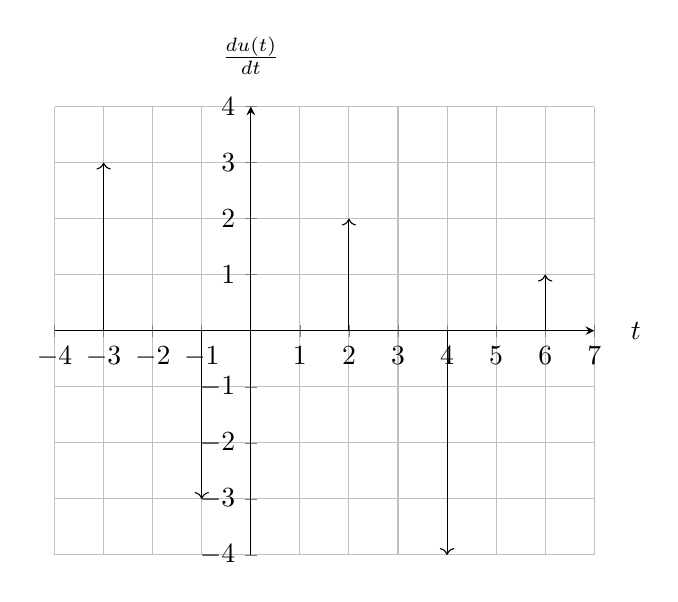
\begin{tikzpicture}[scale=1.0]
           \begin{axis}[
          axis lines=middle,
          xlabel={$t$},
          ylabel={$\frac{du(t)}{dt}$},
          xtick={-4, -3, ..., 7},
          ytick={-4, -3, ..., 4},
          ymin=-4, ymax=4,
          xmin=-4, xmax=7,
          every axis x label/.style={at={(ticklabel* cs:1.05)}, anchor=west,},
          every axis y label/.style={at={(ticklabel* cs:1.05)}, anchor=south,},
          grid,
        ]
           \draw [->] (-3,0) -- (-3, 3);
           \draw [->] (-1,0) -- (-1, -3);
           \draw [->] (2,0) -- (2,2);
           \draw [->] (4,0) -- (4,-4);
           \draw [->] (6,0) -- (6,1);
           \end{axis}
        \end{tikzpicture}
        \caption{$t$ vs. $\frac{du(t)}{dt}$.}
        \label{fig:q6}
    \end{figure}
    
    \end{enumerate}

\item %write the solution of q8
    \begin{enumerate}
    \item
        \begin{enumerate}
        \item Memory: It has memory, for example y[1] = x[0].
        \item Stability: It is stable, because all bounded inputs result in bounded outputs.
        \item Causality: It is not causal, because output depends on future output. y[5] = x[8]
        \item Linearity: We can say it's linear, because superposition holds.\\
        (Superposition means that $y_1(t) + y_2(t) = h(x_1(t) + x_2(t))$.)
        \item Invertibility: It's not invertible, because $x[n] = y[\frac{n+2}{2}]$ is not defined for all values of n.
        \item Time-invariance: We can say that it's time varying. $x[2n-2n_0-2]\neq[2n-n_0-2]$
        \end{enumerate}
    \item 
        \begin{enumerate}
        \item Memory: It has memory, for example $y(2)=2x(0)$
        \item Stability: It's not stable, because bounded inputs does not always create bounded outputs (y(t) depends on t that is unbounded).
        \item Causality: It's causal, because output does not depend on future inputs.
        \item Linearity: It's linear, because superposition property holds.\\
        (Superposition means that $y_1(t) + y_2(t) = h(x_1(t) + x_2(t))$.)
        \item Invertibility: It's not invertible, because $x(t)=\frac{y(2t+2)}{2t+2}$ is not defined for $t = -1$.
        \item Time-invariance: It's time varying. $tx(\frac{t-t_0}{2}-1)\neq(t-t_0)x(\frac{t-t_0}{2}-1)$
        \end{enumerate}
    \end{enumerate}    

\end{enumerate}

\end{document}

